%%%%%%%%%%%%%%%%%%%%%%%%%%%%%%%%%%%%
%% PREAMBLE 
%%%%%%%%%%%%%%%%%%%%%%%%%%%%%%%%%%%%

\documentclass[11pt]{article}

% nice clickable URLs
\usepackage{url}  
\usepackage{amsmath}
\usepackage{graphicx}
\usepackage[utf8]{inputenc}
\usepackage[english]{babel}
\usepackage{color}
% conditional independence
\newcommand{\bigCI}{\mathrel{\text{{$\perp\mkern-10mu\perp$}}}}
\newcommand{\Sara}[1]{{\color{blue} Sara: #1}}

% page margins 
\setlength{\paperwidth}{494pt} % A4
\setlength{\textwidth}{420pt}
\setlength{\hoffset}{-30pt}
\setlength{\oddsidemargin}{-5pt}
\setlength{\paperheight}{846pt} % A4
\setlength{\textheight}{700pt}
\setlength{\voffset}{0pt}
\setlength{\topmargin}{-50pt}
\setlength{\headheight}{0pt}
\setlength{\headsep}{25pt}
\setlength{\parindent}{0pt} % {20pt}
\setlength{\parskip}{4pt plus 2pt minus 1pt}


\begin{document}

%%%%%%%%%%%%%%%%%%%%%%%%%%%%%%%%%%%%
%% HEADING 
%%%%%%%%%%%%%%%%%%%%%%%%%%%%%%%%%%%%
\rule{\textwidth}{1pt}

\textbf{Thesis Project} \hfill 2017
\rule{\textwidth}{1pt}
\vspace*{20pt}

%%%%%%%%%%%%%%%%%%%%%%%%%%%%%%%%%%%%
%% ENTER DETAILS
%%%%%%%%%%%%%%%%%%%%%%%%%%%%%%%%%%%%

% write the homework number in place of "NUM"
\textbf{Assignment 3: Literature draft}

% write your name(s) in place of "NAME(S)"
\textbf{Name:} Alex Khawalid, 10634207\\
\textbf{Supervisor:} Sara Magliacane\\
\today

\section{Problem Definition}
Joint Causal Inference (JCI) is a recently proposed framework that aims at discovering causal relations based on observational and experimental data. Currently JCI has only been tested on simulated data and is exclusively applicable to systems with a small number of variables. The overall goal of JCI is to find out causal relations without extensive experimentation.  
By using observational data as well as experimental data JCI is hypothesised to be able to uncover causal relations for systems in general. 

This thesis project will apply ACID-JCI, an implementation based on Ancestral Causal Inference with Determinism (ACID), to a real-world biological dataset. This requires designing ways to make it scale to a larger number of variables. Solving this scalability problem will involve running JCI multiple times on different subsets of the data. Afterwards a theoretically sound method of combining the models produced by JCI must be applied. The combined model will be compared to other models generated by different methods of causal inference. 

Some of the difficulty in solving this problem lies in the fact that the predicted causal relations are scored by confidence scores and not assigned a probability, which makes the combination of different models a non-trivial task. Furthermore two different models might indicate contradictory relationships between variables. Solving these subproblems will be an important part of creating an algorithm to combine these models.

%  Although this is true in a sense, it sounds a bit reductive. The methods you are going to be using and developing are more general than just for protein signalling networks. These networks are just an example of possible datasets that can be used to discover causal relations. You can probably reuse some things from Assignment 2 here.
% Technically JCI is more like a framework that can be implemented with many different methods, the one we used in the paper and that you will be working on is based on ACID (we call it ACID-JCI in the paper, because we also add some background knowledge, but it's the same method). ACI and ACID are both methods that work with ancestral structures, which are indirect causal relations. There is a definition in the ACI paper and there should be an example in the beginning of the slides.
% \Sara{In general, try to use causal graphs or causal models instead of DAGs or ancestral structures, so you don't need to go in detail. When one refers to a causal DAG it is also usually assumed that you don't have any latent/unobserved variable. When there could be latent variables, different methods use different types of graphs, often also with bidirected edges. We will use ancestral structures, which is yet another type of graph.}
\section{Literature Overview}
\begin{itemize}
    \item \textbf{Joint Causal Inference from Observational and Experimental Datasets}\\
    JCI is a framework used to discover causal relations from observational and experimental data. This paper discusses the advantages it has over other methods of causal inference. It also highlights some problems with faithfulness violations which are caused by deterministic relationships. These are solved using an extension of Ancestral Causal Inference (ACI) called Ancestral Causal Inference with Determinism (ACID). ACID-JCI assumes that the structure it is learning might have latent variables, the output model is an ancestral structure.\cite{jci}
    
    \item \textbf{Ancestral Causal Inference}\\
    To understand why ACID was needed to help JCI to deal with faithfulness violations, ACI, a technique for reconstructing indirect causal relations, must be looked at. ACI is a technique used to discover causal relations. It also allows for the presence of latent variables in a system and produces an ancestral structure. However, the faithfulness violations caused by JCI prevent ACI from being used in the JCI framework. \cite{aci}
    
    \item \textbf{Exact Bayesian structure learning from uncertain interventions}\\
    When talking about the advantages of JCI, the method has to be compared against different methods. One such method was proposed by Eaton and Murphy, this method is a score based method, unlike JCI which is a constraint based method. In this paper Eaton and Murphy applied a technique using Dynamic Programming (DP). The result that this algorithm produces is a DAG. This paper illustrates how they successfully applied this technique and what the results of their research were. \cite{eaton2007exact}
    
    \item \textbf{Causal Discovery from a Mixture of Experimental and Observational Data}\\
    This paper proposes a different score-based method, Local Causal Discovery, which can discover causal relations for a simple causal pattern. The method described in this paper can also take observational and experimental data into account. \cite{cooper1999causal}
    
    \item \textbf{Causal Protein-Signaling Networks Derived from Multiparameter Single-Cell Data}\\
    The data that JCI will be tested on will be obtained from this paper. This paper describes the dataset which will be used and is necessary to understand it. \cite{sachs2005causal}
\end{itemize}

\section{Keywords}
\begin{itemize}
    \item \textbf{Causal Discovery:} A field in statistics which aims to uncover causal relationships.
    \item \textbf{Causal relationships:} A causal relationship is a relationship between variables where one variable is a part of the function which determines the value of the other. % I read this in the book on page 26
    \item \textbf{Constraint Based Causal Discovery:}  A category of methods of causal discovery which use independence tests to uncover causal relationships. 
    % \Sara{this type of methods don't always produce DAGs, and they should not produce deterministic relations. Deterministic relations are a side-effect that happens only in JCI, and it's mostly because we added the intervention variables. I would just drop this last sentence.}
    \item \textbf{Score Based Causal Discovery:} A category of methods of causal discovery which to find the DAG which is most likely to produce the given data.
    \item \textbf{Directed Acyclical Graph:} A Directed Acyclical graph (DAG), is a graph where any path which can be taken from one node to another does not lead back to the node it started at. Furthermore all edges must be directed.
    \item \textbf{Causal DAG:} A DAG in which each edge represents a direct causal relation.
    \item \textbf{Ancestral structure:} A type of DAG which can represent indirect causal relations. In an ancestral structure it is not certain if an edge represents an indirect or direct causal relation. 
    \item \textbf{Observational and Experimental datasets:} An observational dataset is a dataset where no interventions have been used. Conversely an experimental dataset is a dataset where interventions have been used.
    \item \textbf{d-separation:} Two nodes are d-separated if there is no set of adjacent edges which can connect them. This is denoted as $X \perp_d Y$.
    \item \textbf{d-connection:} Two nodes are d-connected if there is a set of adjacent edges which can connect them. This is denoted as $X \not\perp_d Y$.
    \item \textbf{Conditional Independence:} Conditional independence is denoted as $X \bigCI Y \vert \textbf{W}[\mathcal{P}]$. Where X, Y and \textbf{W} are a disjoint set of random variables and $\mathcal{P}$ is their joint probability distribution.
    \item \textbf{Causal Markov Assumption:} ``d-separation in the causal DAG $\mathcal{G}$ implies conditional independence in the observational distribution $\mathcal{P}$''\cite[p.~3]{jci}. For all disjoint sets of variables \textbf{X}, \textbf{Y}, \textbf{W}:
    $$ \textbf{X} \perp_d \textbf{Y} \vert \textbf{W} [\mathcal{G}] \Longrightarrow \textbf{X} \bigCI \textbf{Y} \vert \textbf{W} [\mathcal{P}] $$
    This formula was taken from the paper describing JCI\cite[p.~3]{jci}. In this same paper the formula is also expressed as :
    $$ \textbf{X} \not \bigCI \textbf{Y} \vert \textbf{W}[\mathcal{P}] \Longrightarrow \textbf{X} \not \perp_d \textbf{Y} \vert \textbf{W} [\mathcal{G}] $$\cite[p.~3]{jci}
    \item \textbf{Faithfulness Violations:} ``the inverse of the Causal Markov assumption'', the following formula was taken from the paper about JCI\cite[p.~4]{jci}:
    $$ \textbf{X} \bigCI \textbf{Y} \vert \textbf{W}[\mathcal{P}] \Longrightarrow \textbf{X} \perp_d \textbf{Y} \vert W [\mathcal{G}] $$
\end{itemize}

\begin{figure}[h!]
    \centering
    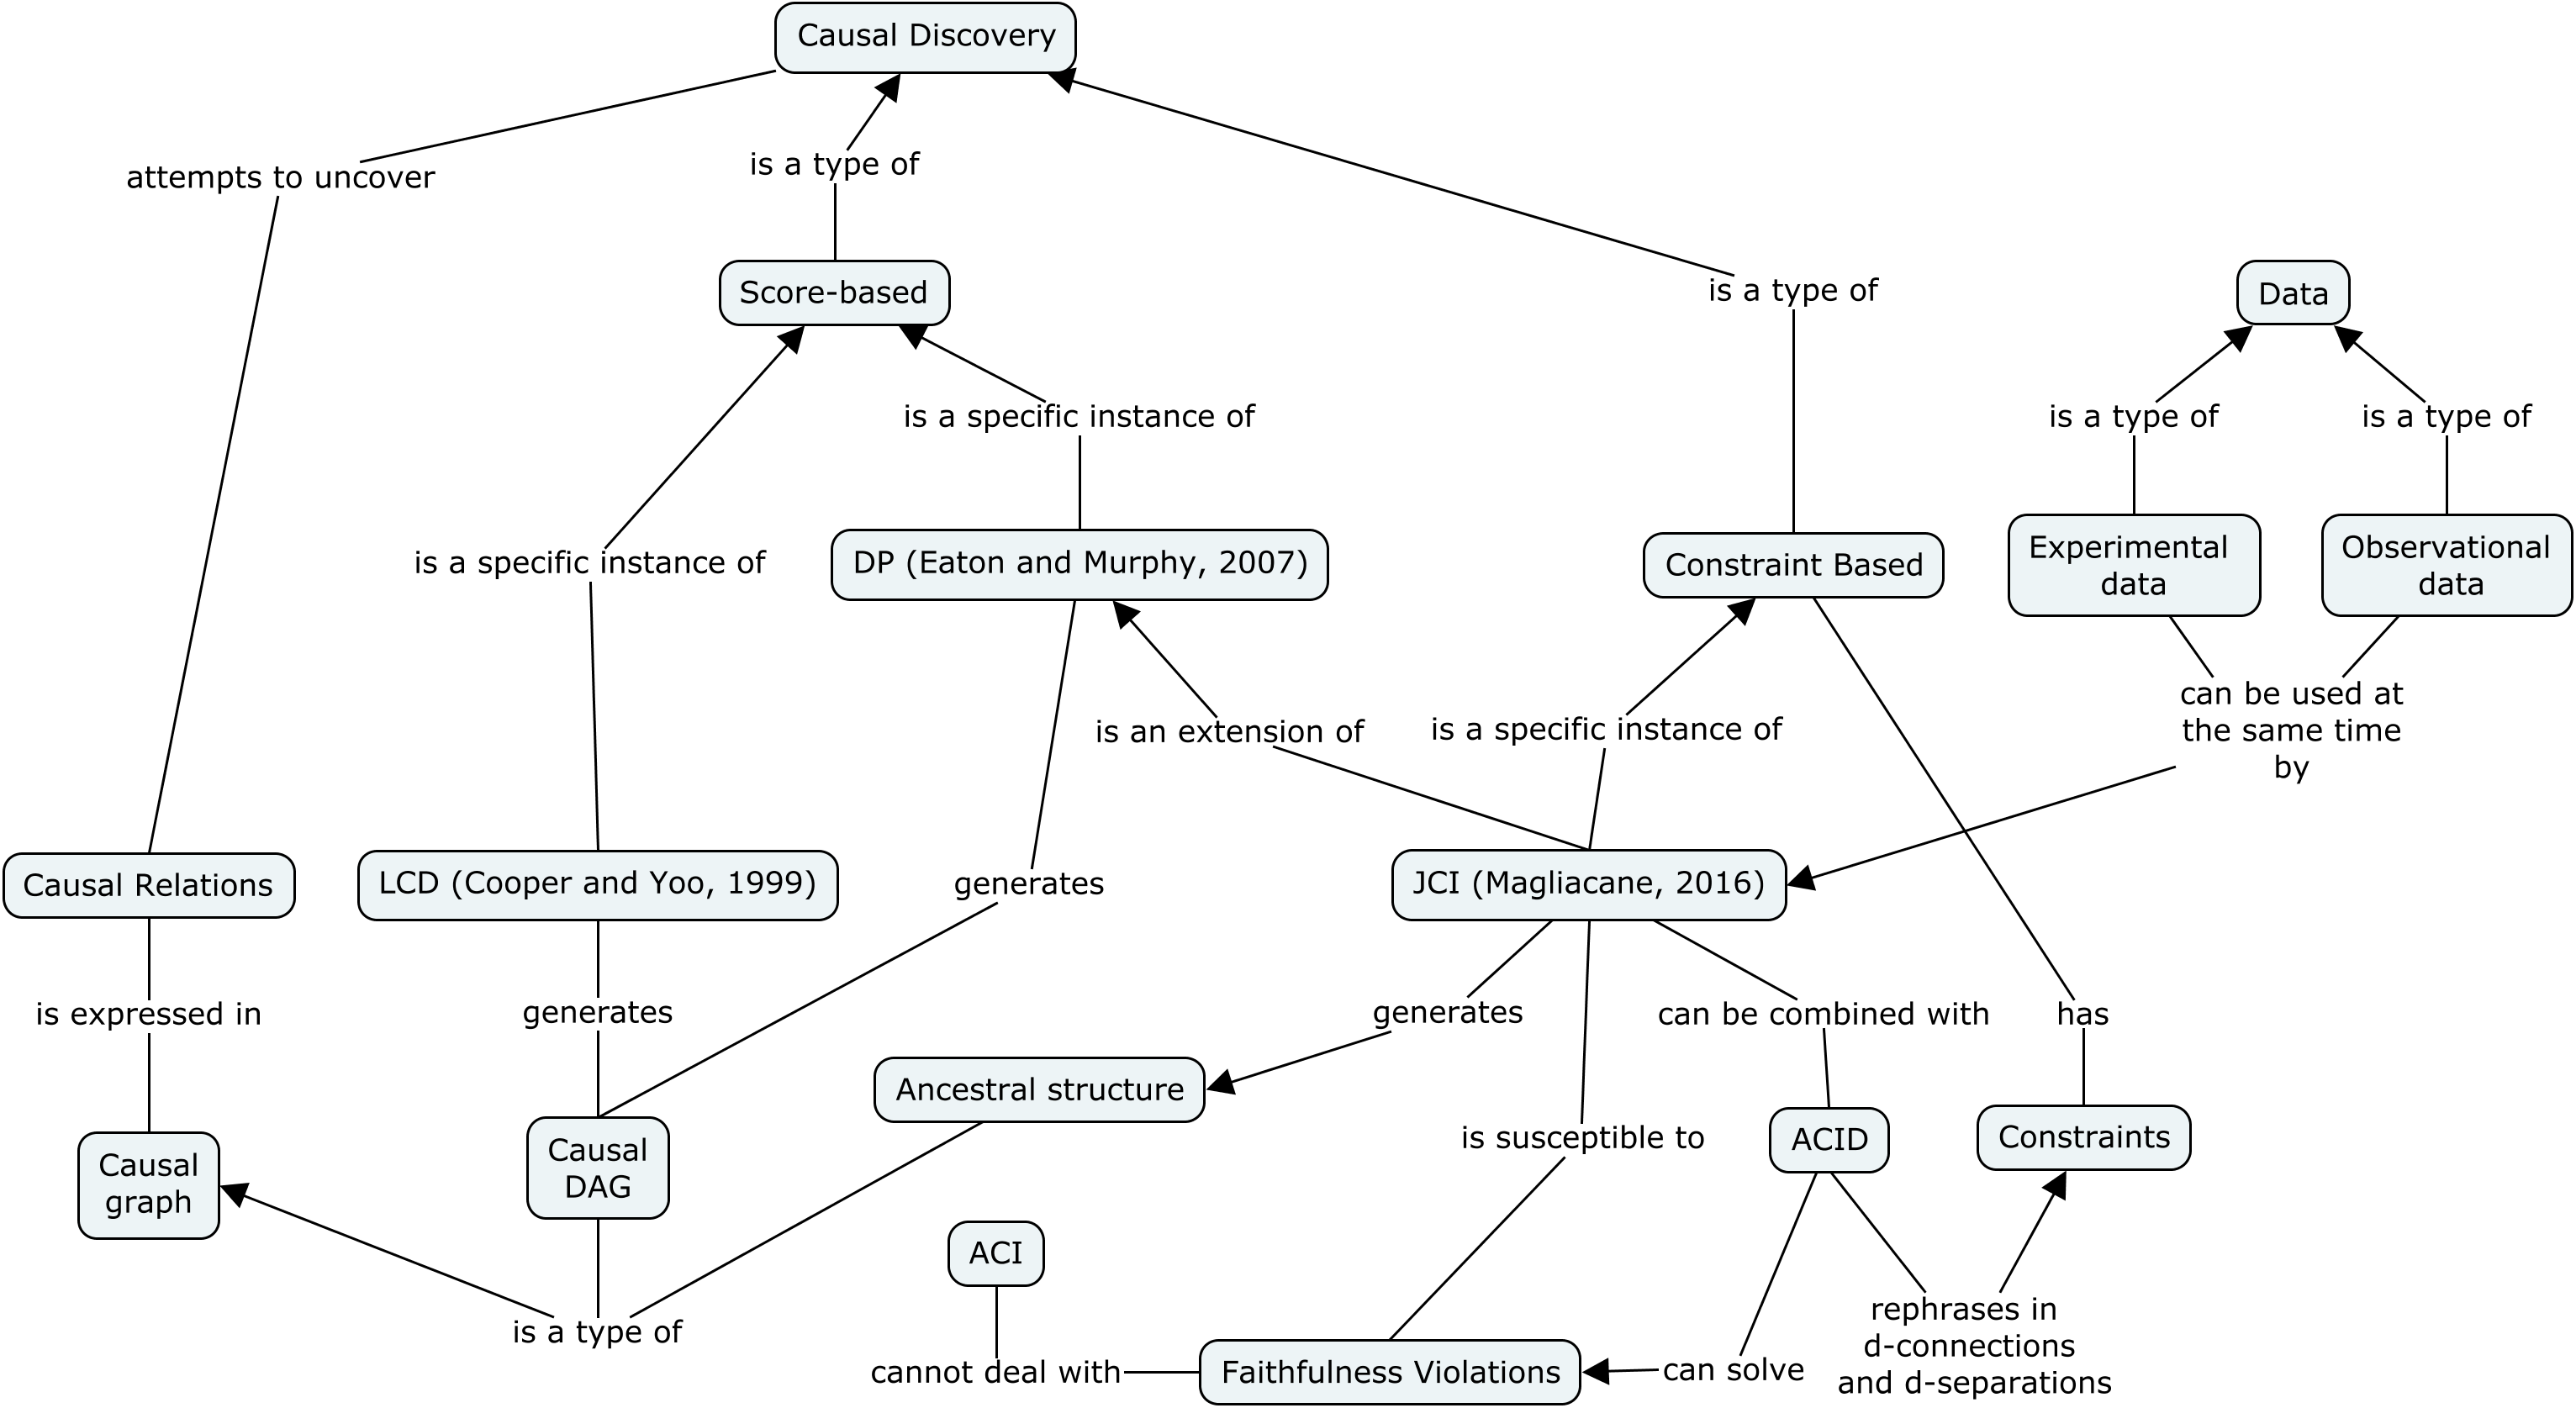
\includegraphics[width=\textwidth]{assignment3_cmap.png}
    \caption{Concept map of thesis topic}
    \label{fig:cmap}
\end{figure}
% % % % % % Assignment

% Make a draft for the literature overview of your thesis topic:

% Create a first draft of your problem definition (in cooperation with your supervisor). Use max. 200 words.

% Create a collection of key words and a concept map for your topic. Characterize the concepts as much as possible and label the relations between them. (You can use CmapTools for your concept map, see RTM below).

% Collect (in cooperation with your supervisor) a minimum of 5 relevant articles. For each article, create a BibTex entry and summarize the most important points and the link to your own project in max. 1/2 page.
% Use these descriptions to create your literature overview draft.
% For more details, see the following items in the Course Documents folder:

% Research Territory Mapping (RTM)
% BibTex
% Referencing scientific articles

\bibliographystyle{abbrv}
\bibliography{ref1} 

\end{document}